\section{Contraction Message Passing}\label{cha:messagePassing}

In this chapter we introduce local contraction passed along tensor clusters to approximatively calculate global contractions.
These message passing schemes provide tradeoffs between efficiency increases and exactness of the global contraction.
We use the CP Decompositions to investigate the asymptotic behavior of the message passing algorithms.



\subsection{Exact Contractions}

%\red{This is the junction tree algorithm!}

We apply Theorem~\ref{the:splittingContractions} to split a contraction into subcontractions, which are consecutively performed.

% Message Passing
Contractions can be performed partially, and the result passed to the rest of the network as a message.

\subsubsection{Construction of Cluster Graphs}

% Cluster Graphs
\begin{definition}[Cluster Graph]
	Given a tensor network $\extnet$ a cluster partition is a partition of the tensor network into $n$ clusters, by a function
		\[ \alpha : \edges \rightarrow [n] \, . \]
	The clusters are with tensors decorated edge sets $\enc = \{\edge \, : \, \alpha(\edge) = i\}$ with variables $\nodes_i = \bigcup_{\edge \in \enc} \edge$.
	The clusters form a graph where edges between $\enc$ and $C_j$ exist, when the node sets $\nodes_i$ and $\nodes_j$ are not disjoint.
	In this case, we define separation sets $S_{i,j}=\enc\cup C_j$
\end{definition}

\begin{theorem}
	Given a tensor network $\extnet$ and a cluster graph.
	We then define for each cluster the node set
		\[ \tilde{\nodes}_i = \bigcup_{j\neq i} \nodes_j \]
	and have
		\[ \contractionof{\extnet}{\catvariableof{\secnodes}} = 
		\contractionof{
			\{ \contractionof{ \tnetof{\enc} }{\nodes_i \cap (\tilde{\nodes}_i\cup\secnodes)}  : i \in [n]\}
		}{\catvariableof{\secnodes}}  \, . \]
\end{theorem}
\begin{proof}
	By Theorem~\ref{the:splittingContractions} applied for each cluster seen as a subgraph.
\end{proof}



\subsubsection{Message Passing to calculate contractions}

% Cluster Graphs
Having a hypergraph $\graph$, we iteratively apply Theorem~\ref{the:splittingContractions} and call the $\graph_2$ a cluster.
When iterating until $\graph$ is empty, we get a cluster graph, where all tensors are assigned to a cluster.


% Cluster Trees -> Clique Trees in Koller Book
When the cluster are a polytree, that is a union of disjoint trees, we define messages between neighbored clusters $\enc$ and $\secenc$ with $\secenc\prec\enc$ by the contractions

\begin{align}
	\upmes{j}{i} = \contractionof{\{\upmes{\tilde{j}}{j} \, : \,  \thirdenc \prec \secenc\} \cup \tnetof{\secenc}}{\catvariableof{\nodes_i\cap \nodes_j}} \, .
\end{align}
and
\begin{align}
	\downmes{i}{j}  = \contractionof{\{\downmes{\tilde{j}}{i} \, : \,  \enc \prec  \thirdenc\} \cup \tnetof{\enc}}{\catvariableof{\nodes_i\cap \nodes_j}} \, .
\end{align}


We note, that the messages are well defined by these recursive equations, exactly when the cluster graph is a polytree.
%Since messages are recursively defined, we need the tree structure to ensure well-definedness.


\begin{lemma}
	When the cluster graph is a tree, we have for neighbored clusters $\enc$ and $\secenc$ with $\secenc\prec\enc$
		\[ \upmes{\secclusterenumerator}{\clusterenumerator} 
		= \contractionof{\{\tnetof{\thirdenc} \, : \, \thirdenc \prec \secenc \}}{\catvariableof{\nodes_i\cap\nodes_j}}   \]
	and
		\[ \downmes{\clusterenumerator}{\secclusterenumerator}
		= \contractionof{\{\tnetof{\thirdenc} \, : \, \enc \prec \thirdenc \}}{\catvariableof{\nodes_i\cap\nodes_j}}  \, . \]
\end{lemma}
\begin{proof}
	By induction over the cardinality of the preceding clusters.
	\paragraph{$n=1$}: Only a single cluster before, therefore trivial.
	\paragraph{$n+1\rightarrow n$}: Assuming the statement holds for up to $n$ preceding clusters, let there be $n+1$ preceding clusters.
	Then Theorem~\ref{the:splittingContractions} splits contractions into terms, which are by inductive assumption the messages.
\end{proof}


\begin{theorem}
	When the cluster graph is a tree, then we have for each cluster $\enc$ with neighbors $N(\clusterenumerator)$
%	Then for each clique we have the conditional probability of its variables being the contraction of the messages with the cliques cores, that is
	\begin{align}
		\contractionof{\extnet}{\nodes_i} = 
		\contractionof{
			\{ \upmes{\secclusterenumerator}{\clusterenumerator}  \, : \, j \in N(i) , \, \secenc\prec\enc \}  \cup 
			\{ \downmes{\secclusterenumerator}{\clusterenumerator}  \, : \, j \in N(i),  \, \enc\prec\secenc \} \cup \tnetof{\enc}
		}{\nodes_i} \, .
	\end{align}
\end{theorem}
\begin{proof}
	By Theorem~\ref{the:splittingContractions} we split into contractions of the clusters up and down of the respective neighbors and apply the above lemma.
\end{proof}





\subsubsection{Variable Elimination Cluster Graphs}


\begin{remark}[Construction of Cluster Graphs by Variable Elimination]
	% Build a cluster graph
	Following an elimination order of the colors, mark those tensors containing the colors, which have not been marked before, as the cluster.
	% Extension to clique tree
	A clique tree can be constructed by these cluster, when iterating through the clusters and either connect them to previous disconnected clusters or leave the current cluster disconnected.
	Add the disconnected clusters with the current cluster in case there are overlaps of their open colors.
	If the disconnected cluster added has more open colors, 
\end{remark}


\subsubsection{Bethe Cluster Graphs}


\begin{figure}[h]
\begin{center}
	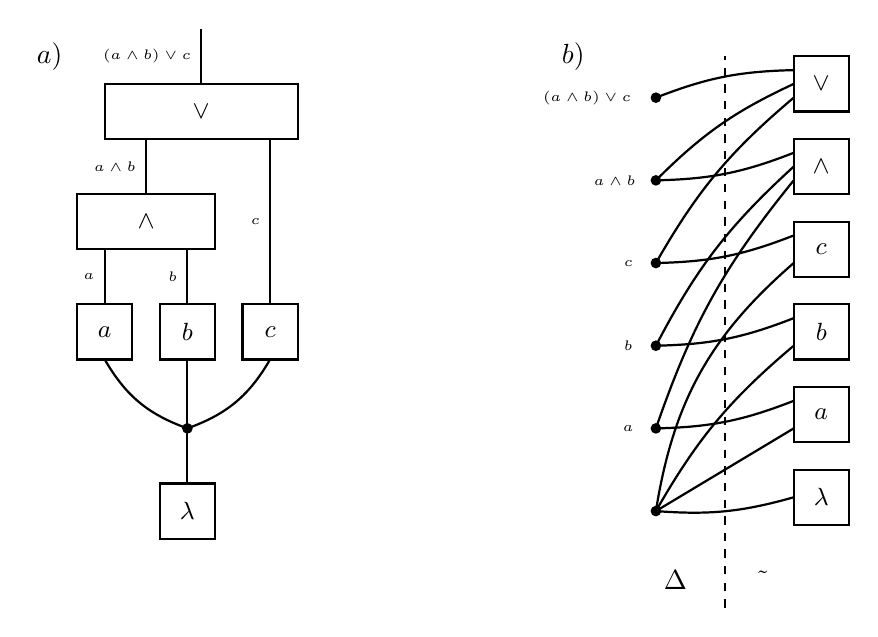
\begin{tikzpicture}[scale=0.35, thick] % , baseline = -3.5pt




\begin{scope}[shift={(23,0)}]

\node[anchor=center] (text) at (-6,8) {$b)$};

\draw (2,8) rectangle (4,6);
\node[anchor=center] (text) at (3,7) {\small $\bencodingof{\lor}$};

\draw (2,5) rectangle (4,3);
\node[anchor=center] (text) at (3,4) {\small $\bencodingof{\land}$};

\draw (2,2) rectangle (4,0);
\node[anchor=center] (text) at (3,1) {\small $\datacoreof{c}$};

\draw (2,-1) rectangle (4,-3);
\node[anchor=center] (text) at (3,-2) {\small $\datacoreof{b}$};

\draw (2,-4) rectangle (4,-6);
\node[anchor=center] (text) at (3,-5) {\small $\datacoreof{a}$};

\draw (2,-7) rectangle (4,-9);
\node[anchor=center] (text) at (3,-8) {\small $\lambda$};


\draw[fill] (-3,-8.5) circle (0.15cm);
\node[anchor=center] (text) at (-4,-8.5) {\tiny $\indexset$};

\draw[] (-3,-8.5) to[bend left=-10]  (2,-8);
\draw[] (-3,-8.5) to[bend left=0]  (2,-5.5);
\draw[] (-3,-8.5) to[bend left=10]  (2,-2.5);
\draw[] (-3,-8.5) to[bend left=20]  (2,0.5);


\draw[fill] (-3,-5.5) circle (0.15cm);
\node[anchor=center] (text) at (-4,-5.5) {\tiny $a$};

\draw[] (-3,-5.5) to[bend left=-10]  (2,-4.5);
\draw[] (-3,-5.5) to[bend left=10]  (2,3.5);

\draw[fill] (-3,-2.5) circle (0.15cm);
\node[anchor=center] (text) at (-4,-2.5) {\tiny $b$};

\draw[] (-3,-2.5) to[bend left=-10]  (2,-1.5);
\draw[] (-3,-2.5) to[bend left=10]  (2,4);

\draw[fill] (-3,0.5) circle (0.15cm);
\node[anchor=center] (text) at (-4,0.5) {\tiny $c$};

\draw[] (-3,0.5) to[bend left=-10]  (2,1.5);
\draw[] (-3,0.5) to[bend left=10]  (2,6.5);

\draw[fill] (-3,3.5) circle (0.15cm);
\node[anchor=center] (text) at (-4.5,3.5) {\tiny $a\land b$};

\draw[] (-3,3.5) to[bend left=-10]  (2,4.5);
\draw[] (-3,3.5) to[bend left=10]  (2,7);

\draw[fill] (-3,6.5) circle (0.15cm);
\node[anchor=center] (text) at (-5.5,6.5) {\tiny $(a\land b)\lor c$};

\draw[] (-3,6.5) to[bend left=10]  (2,7.5);


\draw[dashed] (-0.5,-12) -- (-0.5,8);

\node[right] (text) at (0.5,-11) {$\tilde{\edges}$};
\node[left] (text) at (-1.5,-11) {$\Delta$};

\end{scope}


\node[anchor=center] (text) at (-2,8) {$a)$};

\newcommand{\conposseldec}{3,-5.5}

\draw[fill] (\conposseldec) circle (0.15cm);
\draw (\conposseldec) -- (3,-7.5) node[midway, right] {\tiny ${\indexset}$}; % Unclear, whether this is the best notation!
\draw[] (2,-7.5) rectangle (4, -9.5);
\node[anchor=center] (text) at (3,-8.5) {\small $\lambda$};

\draw[] (0,1) -- (0,-1) node[midway,left] {\tiny $a$};
\draw (-1,-1) rectangle (1, -3);
\node[anchor=center] (text) at (0,-2) {\small $\datacoreof{a}$};
\draw[] (0,-3) to[bend right=20] (\conposseldec);


\draw[] (3,1) -- (3,-1) node[midway,left] {\tiny $b$};
\draw (2,-1) rectangle (4, -3);
\node[anchor=center] (text) at (3,-2) {\small $\datacoreof{b}$};
\draw[] (3,-3) to[bend right=0]  (\conposseldec);


\draw[] (6,5) -- (6,-1) node[midway,left] {\tiny $c$};
\draw (5,-1) rectangle (7, -3);
\node[anchor=center] (text) at (6,-2) {\small $\datacoreof{c}$};
\draw[] (6,-3) to[bend left=20]  (\conposseldec);


\draw[] (1.5,5) -- (1.5,3) node[midway,left] {\tiny $a \land b $};
\draw (-1,3) rectangle (4, 1);
\node[anchor=center] (text) at (1.5,2) {\small $\bencodingof{\land}$};


\draw[] (3.5,9) -- (3.5,7) node[midway,left] {\tiny $(a \land b) \lor c $};
\draw (0,7) rectangle (7, 5);
\node[anchor=center] (text) at (3.5,6) {\small $\bencodingof{\lor}$};

%\draw[] (6,1) to[bend left=20]  (\conposseldec);


		


\end{tikzpicture}
\end{center}
\caption{Example of a Bethe Cluster Graph.
	a) Example of a Tensor Network $\tnetof{\graph}$, which represents the by $\lambda$ averaged evaluation of the formula $(a\land b)\lor c$ on data $\datamap$.
	b) Corresponding Bethe Cluster Hypergraph, which dual is bipartite by the sets $\Delta$ and $\tilde{\edges}$.
	}
\label{fig:betheDataExample} 
\end{figure}

By adding delta tensors to each node $\node\in\nodes$ and defining its leg variables by $\node^{\edge}$ for $\edge\in\edges$.
We mark each such delta tensor by a cluster in $\Delta^{\graph}$, as defined in the following (see also Figure~\ref{fig:betheDataExample}).

\begin{definition}
	Given a tensor network $\tnetof{\graph}$ on a decorated hypergraph $\graph$, we define the Bethe Cluster Hypergraph $\secgraph$ as
	$(\secnodes, \secedges \cup \Delta^{\graph})$ where we have
	\begin{itemize}
		\item Recolored Edges $\secedges = \{\tilde{\edge} \, : \, \edge\in \edges\}$ where $\tilde{\edge} = \{\node^{\edge} \, : \, \node\in\edge\}$, which decoration tensor has same coordinates as $\hypercoreof{\edge}$
		\item Nodes $\secnodes = \bigcup_{\edge\in\edges}\tilde{\edge}$ %$\secnodes = \bigcup_{\edge\in\edges}\{\node^{\edge} \, : \, \node\in\edge \}$ 
		\item Delta Edges $\Delta^{\graph} =  \big\{ \{\node^{\edge} \, : \, \edge\ni\node \} \, : \, \node\in\nodes \big\} $, each of which decorated by a delta tensor $\delta^{\{\node^{\edge} \, : \, \edge\ni\node \}}$
	\end{itemize}
\end{definition}

By \lemref{lem:deltification} this construction does not change contractions.

% Dual graph
The dual is bipartite, since any variable appears exactly in one cluster in $\secedges$ and in one cluster of $\Delta^{\graph}$.
This further makes the dual of the Bethe Cluster Hypergraph a proper graph (i.e. edges consistent of node pairs). 





\subsubsection{Computational Complexity}

\red{Tree-width here.}

Naive execution of $\contractionof{\tnetof{\graph}}{\secnodes}$: $\prod_{\node\in\nodes} \catdimof{\node}$ many products are built and summed up.
When splitting contractions into local subcontractions, the product can be turned into sums with tremendous decrease in complexity.









\subsection{Approximate Contractions}

We ignore that cluster graphs are not trees and perform contraction message passing along neighbored clusters.
For the contraction of basis tensor networks, this scheme still provides the exact contraction.

\subsubsection{Exact Message Passing for Directed and Binary Contractions}


%% Function Composition Perspective
A Tensor Network of directed and binary cores represents the evaluation of composed functions.
In a Message Passing Perspective each component (let us call them neurons) can be evaluated, when the evaluation of the ancestor neurons are known.

\begin{lemma}\label{lem:diracConBasis}
	\red{Required? Basis vector factorization suffices?}
	For any collection of categorical variables $\shortcatvariables$ with identical dimension and any $\catindexofin{0}$ we have
		\[ \sbcontractionof{\delta[\catvariableof{0},\ldots,\catvariableof{\catorder-1}]}{\indexedcatvariableof{0},\catvariableof{1},\ldots,\catvariableof{\catorder-1}} 
		= \bigotimes_{\catenumerator\in\{1,\ldots,\catorder-1\}} \onehotmapofat{\catindexof{0}}{\catvariableof{\catenumerator}} \, . \]
\end{lemma}
\begin{proof}
	Directly by sum decomposition of delta tensors.
\end{proof}

\begin{theorem}
	Let $\tnetof{\graph}$ be a tensor network on a directed acyclic hypergraph $\graph$, such that each tensor is Boolean and directed, and such that each variable is appearing only once as an outgoing variable of a hyperedge.
	We build a cluster graph by storing each edge as a cluster and use the topological order on $\graph$.
	%We denote the scalar messages on the edges with no outgoing variables a single propagation of messages along the direction of the Bethe Cluster Graph by $\delta^{\edge}$ 
	%Then they coincide with the exact contractions leaving the variables of the edge open.	
	Then
		\[ \upmes{j}{i} = \contractionof{\tnetof{\graph}}{\catvariableof{\nodes_i\cap\nodes_j}} \, . \]
\end{theorem}
\begin{proof}
\red{Lemma above needed?}
	By using that each message is a basis vector (Using Theorem~\ref{the:conditionalContractionPreservation} in an induction argument) and can thus be splitted into the product of multiple copies.

	% Reducing to downcore
	Any hypercore, which is not a precessor to $\hypercoreof{\edge_{\clusterenumerator}}$ can be omitted from the contraction by a root-stripping argument using its directionality.
	Therefore we have
	\begin{align*}
		\contractionof{\tnetof{\graph}}{\catvariableof{\nodes_i\cap\nodes_j}}
		= \contractionof{\{\hypercoreof{\edge_{\thirdclusterenumerator}} \, : \, \edge_{\thirdclusterenumerator} \prec \edge_{i} \}}{\catvariableof{\nodes_i\cap\nodes_j}} \, . 
	\end{align*}

	We then replace each variable which is appearing more than once in outgoing legs by a delta tensor, which does not change the contraction by \lemref{lem:deltification}.
	%When there are undirected loops in the network beyond the cluster, we apply \lemref{lem:diracConBasis} to replace the variable by its copies and a delta tensor.
	
	We then follow a leaf stripping argument and apply Theorem~\ref{the:splittingContractions} iteratively on the remaining leaves. 
	Along that line, the leave and its successors are contracted.
	The contraction is a basis vector and can therefore be represented as an outer product of basis vectors.

\end{proof}



When replacing $\onehotmapof{\catindexof{0}}$ by an arbitrary vector in \lemref{lem:diracConBasis} we have
	\[ \sbcontractionof{\delta[\catvariableof{0},\ldots,\catvariableof{\catorder-1}], V[\catvariableof{0}]}{\catvariableof{1},\ldots,\catvariableof{\catorder-1}} 
		\neq \bigotimes_{\catenumerator\in\{1,\ldots,\catorder-1\}} V[{\catvariableof{\catenumerator}}]  \, . \]
Therefore, the messages will in general differ from the exact contractions.
To provide intuition of what happens in this case, let us take the following cases into account:
\begin{itemize}
	\item $\lambda\cdot\onehotmapof{\catindex}$ sent multiple times: Result gets a factor of $\lambda^{\# \text{copies}}$ compared with the exact contraction.
	\item $\onehotmapof{\catindex}+\onehotmapof{\tilde{\catindex}}$: Result is the exact contraction added by the crossterms of sending $\onehotmapof{\catindex}$ in one and $\onehotmapof{\tilde{\catindex}}$ in the other direction.
\end{itemize}	



\subsubsection{Case of Matrices}

\red{Here a toy example of cycling messages starting with $\ones$.
When normating the messages, the maximal singular vectors will be dominant.}

We investigate the Bethe message passing for a tensor network consisting of a single matrix.

\begin{theorem}
	The stable messages are the linear subspace of the maximal singular values of the fixed core $\hypercore$.
\end{theorem}
\begin{proof}
	Having a Singular Value Decomposition of $\hypercore$ and decompose the messages in the orthonormal system of the respective singular vectors.
\end{proof}


For the propagation of $a$ and $b$ on binary $\exformula(a, b)$ starting with trivial messages of $a$ and $b$ the above theorem implies:
\begin{itemize}
	\item Case of single possible world: Exact 
		$\exformula(a, b) \in \{ a \land b, a \land \lnot b, \lnot a \land b, \lnot a \land \lnot b \}$
		Messages are after first iteration exact
	\item Case of two possible worlds and $\exformula(a, b) \in \{ a \Leftrightarrow b, a \Leftrightarrow \lnot b, \lnot a \Leftrightarrow b, \lnot a \Leftrightarrow \lnot b \}$. 
		In this situation any start message is stable and determines the other.
	\item Case of two possible worlds and $\exformula(a, b) \in \{ a, b, \lnot a, \lnot b\}$.
		In this situation one stable message is determined by the specified atom and the other is always stable.
	\item Case of  three possible worlds: Approximative (exact: $1/3, 2/3$, approximative: $1-golden ratio, golden ratio$
	\item Case of four possible worlds: Exact ($\ones$) 
\end{itemize}


\subsubsection{Case of Tensors}

Let there now be a single tensor of arbitrary order.
When the tensor is not ODECO, we cannot find a CP-Decomposition with leg vectors building an orthonormal system in the respective leg spaces.
This prohibits direct application of the same techniques in the case of a matrix, which is always ODECO.



\subsection{Basis Calculus}

Message Passing of directed and binary message by relational encoding of functions can be interpreted as function evaluation.
This is because any relational encoding of a function, the decomposition
\begin{align*}
	\rencodingof{\exfunction} = \sum_{y \in \imageof{\exfunction}} ( \sum_{i: \exfunction(i)=y}\onehotmapof{i} )  \otimes \onehotmapof{y}
\end{align*}
is a SVD of the matrification of $\rencodingof{\exfunction}$ with respect to incoming and outgoing legs.


Passing a message $\onehotmapof{i}$ in direction thus gives the message $\onehotmapof{\exfunction(i)}$.


%After having established a one-to-one connection between the directed and binary tensors with the encoding of functions, we now interpret contractions as evaluations of the respective functions.
%Applying this insight iteratively on composed functions we show the following theorem.

\begin{remark}[Basis Calculus as Message Passing]
	Given a tensor network of directed and binary tensor cores $\hypercoreof{\edge}$, each representing a function $\exfunction^{\edge}$.
	When there are not directed cycles, we define the compositions of $\exfunction^{\edge}$ to be the function $\exfunction$ from the nodes $\nodes_1$ not appearing as incoming nodes to the nodes $\nodes_2$ not appearing as outgoing nodes in an edge.
	Choosing arbitrary $\catindexof{\node}\in[\catdimof{\node}]$ for $\node\in\nodes_1$ we have
	\begin{align*}
		\contractionof{\{\hypercoreof{\edge} \, : \edge\in\edges\}}{\nodes_2} = \onehotmapof{\exfunction(\catindexof{\node} \, : \, \node\in\nodes_1)}\, . 
	\end{align*}
\end{remark}
%\begin{proof}
%	Use a message passing argument for each function $\exfunction^{\edge}$.
%\end{proof}




\subsection{Applications}

% Application: Dynamic programming
When queries share same parts, can perform their contraction using dynamic programming.
For conditional probability queries, which variables are the clusters of a cluster tree, this results in belief propagation.


